\documentclass[fleqn,xcolor={usenames,dvipsnames}]{beamer}
\usepackage{amsmath} % {amssymb,amsfonts}
% \usepackage{colortbl}

\usepackage{comment}

% \usepackage{booktabs, multicol, multirow, adjustbox}
\usepackage{array, adjustbox,url}
\usepackage{pifont,marvosym} % wasysym

\usepackage{multimedia}
\usepackage[normalem]{ulem}
\usepackage{framed,color,ragged2e}
\usepackage[absolute,overlay]{textpos}
\definecolor{shadecolor}{rgb}{0.8,0.8,0.8}
\usetheme{boxes}
\setbeamertemplate{navigation symbols}{}
\usepackage{xcolor}
\usepackage{tikz}
\usetikzlibrary{shapes,arrows}
\usetikzlibrary{positioning}
\usetikzlibrary{calc}
% \usetikzlibrary{cd}
\usepackage[normalem]{ulem}

% ref. http://tex.stackexchange.com/a/84763
% \usepackage{pgfpages}
% \setbeameroption{show notes}
% \setbeameroption{show notes on second screen=right}


\newcolumntype{R}[2]{%
    >{\adjustbox{angle=#1,lap=\width-(#2)}\bgroup}%
    l%
    <{\egroup}%
}
\newcommand*\rot{\multicolumn{1}{R{45}{1em}}}% no optional argument here, please!


\title{Xolotl}
\subtitle{A compact mixnet format with stronger forward secrecy and hybrid anonymity}
% Now we have to build a GNU one!

\author[Burdges]{Jeff Burdges}
\institute{
  
\includegraphics[scale=0.2]{../logos/gnunet-logo.pdf}

  \vfill
  
\includegraphics[scale=0.2]{../logos/inria.pdf}
}
\date{28.6.2015}


\def\Z{\mathbb{Z}}


\begin{document}


{\setbeamertemplate{footline}{}
\begin{frame}
\titlepage
\end{frame}
}
\setcounter{framenumber}{0}



\begin{frame}{Asynchronous messaging aka E-mail}
Email with GnuPG provides authenticity and confidentiality...
  \begin{itemize}
  \item ... but fails to provide forward secrecy, aka key erasure,
  \item ... and fails to {\em protect meta-data}
  \end{itemize} 
\end{frame}


% \note{
% Compromise between cypher-punk style vs. rigorous academic style.
% Explain forward secrecy as compromise window.
% Comments on tension between key erasure and protecting meta-data.
% }


% Mexican walking fish
% salamander 
% gills resemble trees
% related to tiger salamander 
% neoteny metamorposis into similar salamander if given enough iodine or hormones 

\begin{frame}{Axolotl ratchet by Trevor Perrin and Moxie Marlinspike}
\begin{columns}[T]
\column{0.6\textwidth}
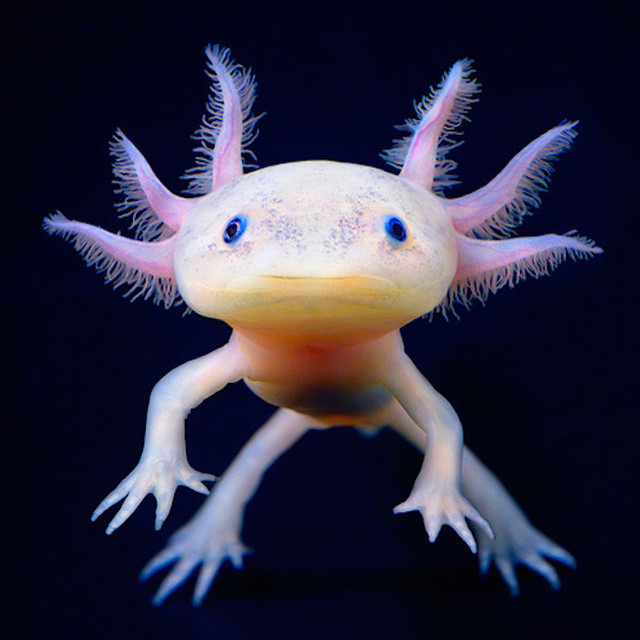
\includegraphics[width=0.8\textwidth]{../pics/axolotl_animal-1.jpg}

Approach: \\
\hspace*{2pt} Run DH whenever possible \\
% \hspace*{5pt} 2-step vs 3-step \\
\hspace*{2pt} Iterate key by hashing otherwise 

% \onslide<2>{
\bigskip
Neutral against Shor's algorithm \\
 \hspace*{2pt} running on a quantum computer. 
% }

\column{0.4\textwidth}
\includegraphics[width=\textwidth]{../pics/axolotl_diagram}
% \vspace*{-20pt}
% \includegraphics[width=0.95\textwidth,trim={0 0 0 47},clip]{axolotl_diagram}
\end{columns}
\end{frame}
% \onslide<2>{
% \begin{quote}
% ``[Axolotl] combines the .. forward secrecy [of] a hash iteration ratchet
% like SCIMP [with the] future secrecy .. of a DH ratchet like OtR'' % \\
% \hfill --- Moxie Marlinspike % (TextSecure)
% }


\begin{comment}
\begin{frame}{Axolotl questions}

Suggested questions on Axolotl during lunch, dinner, etc. : 

\medskip
\begin{itemize}
\item Just ``neutral'' against Shor's algorithm sounds weak.  \\ 
  Can one offer post-quantum forward-secrecy? \\ \medskip
\item How does one authenticate?  Is it deniable? \\ \medskip
\item I heard that punctured encryption adds key erasure to \\
  ordinary public key cryptography like GnuPG? \\
\end{itemize}

\end{frame}
\end{comment}

% Metadata : entropique2015.tex

% Tor : ...

\begin{frame}[t]{Anonymity requires latency}
\begin{columns}[T]
\column{0.8\textwidth}
\hspace*{20pt} Can we just improve Tor?

\medskip

\hspace*{5pt} Tor is inherently vulnerable to correlation attacks \\
 \hspace*{10pt} {\em because} it must deliver many packets quickly.

\bigskip 

% Cryptography works, but 
\hspace*{5pt} Anonymity loves unrealistic ideals like

\column{0.2\textwidth}

\includegraphics[width=\textwidth]{../pics/tor/tor_onion}
% \vspace*{-20pt}
% \includegraphics[width=0.95\textwidth,trim={0 0 0 47},clip]{axolotl_diagram}
\end{columns}
\smallskip
\hspace*{1pt} ``All users are online all the time using constant bandwidth.''

\bigskip
\pause

\noindent We must therefore build applications to
\begin{itemize}
\item be tolerant to high latency, while still
\item being compelling to \sout{the anonymity set} users.
\end{itemize}

\smallskip

We do need an anonymizing transport that handles latency well, \\
\hspace*{2pt} only asynchronous mix networks appear realistic, \\
\hspace*{2pt} due to $O(n^2)$ scalling of bandwidth or computation.

\end{frame}


\begin{comment}
\begin{frame}[t]{Onion Routing vs Mix Networks vs ...}

Anonymizing transports for spherical cows :
\begin{itemize}
\item Dining Cryptographers Networks (DC-nets) \\
 \hspace*{2pt} Aims for even lower latency. $O(n^2)$ bandwidth
\item Private Information Retrieval (PIR) \\
 \hspace*{2pt} Highly application specific.  $O(n^2)$ bandwidth/computation
\item Verifiable mix networks \\
 \hspace*{2pt} Expose packet dropping attacks. $O(n^2)$ computation
\end{itemize}

\end{frame}
\end{comment}


\begin{frame}[t]{Onion Routing vs Mix Networks vs ...}

Anonymity tools need ``onion encryption'' and some routing, but..

\bigskip

Onion routing means progressively establishing a fixed channel, \\
% \hspace*{2pt} 
negotiating a forward secure ephemeral key exchange with each hop \\
\begin{itemize}
\item[Good] Stronger forward secrecy.  Inherently flexible.
\item[Bad] Easy correlation attacks.
\end{itemize}

\medskip

Mix networks encodes all routing and key material into one packet
\begin{itemize}
\item[Good] Much better against correlation attacks.
\item[Bad] Relays cannot use ephemeral key material. 
\item[Mixed] Less flexible, facilitating security analysis. \\
  New protocol :  No TCP, UDP, etc.
\end{itemize}

\medskip\pause
Email handicapped past mix network efforts like Mixminion \\
 \hspace*{10pt} {\bf Do not attempt to support email!}

\end{frame}


\begin{frame}{Sphinx by George Danezis and Ian Goldberg}

\begin{center}

\includegraphics[width=0.8\textwidth]{../pics/Sphinx}
% Mixnets use cryptography in mysterious ways

Sphinx is a packet format for an asynchronous mix network. 

\end{center}
\end{frame}


% \begin{comment}
\begin{frame}{Sphinx by George Danezis and Ian Goldberg}
Sphinx is provably secure in the universal composability model \\
\hspace*{2pt} [Camenisch \& Lysyanskaya '05, Canetti '01]
\begin{enumerate}
\item Provides correct onion routing
\item Integrity, meaning immunity to long-path attacks
\item Security, including \\
\hspace*{2pt} wrap-resistance{\small $^*$} and \\
\hspace*{2pt} indistinguishability of forward and reply messages
\item[] Replay protection implemented by Bloom filter
\end{enumerate}

\bigskip

And Sphinx is far more compact than alternatives.

% Ask later about the caveats..

\bigskip

{\small $^*$ Wrap-resistance helps prevent nodes from acting as decryption oracles.}
\end{frame}
% \end{comment}


\begin{frame}{Sphinx by George Danezis and Ian Goldberg}
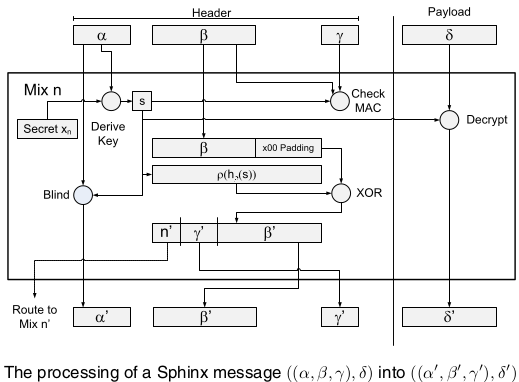
\includegraphics[width=\textwidth]{../pics/Sphinx-diagram}
\end{frame}
% LIONNESS???


\def\mathcomma{}

% \begin{comment}
\begin{frame}{Build a Sphinx header}
First, select a sequence of $\nu$ nodes $n_i$ with keys $X_i = x_i G$ for $i<\nu$,
 an initial private scalar $a_0$, and
 the public curve point $\alpha_0 = a_0 G$.
Now recursively define
\[ \begin{aligned}
\textrm{shared secret}\quad
 s_i &:= a_i X_i = x_i \alpha_i \mathcomma \\
\textrm{blinding factor}\quad
 b_i &:= H(\alpha_i,s_i) \mathcomma \\
\textrm{next private key}\quad
 a_{i+1} &:= b_i a_i \mathcomma \\ % \quad\textrm{and} \\
\textrm{next public key}\quad
 \alpha_{i+1} &:= b_i \alpha_i \quad\textrm{for $i < \nu$.} \\
\end{aligned} \]
% Our $i$th node replaces $\alpha_i$ by $\alpha_{i+1}$.

Next, ...

\end{frame}
% \end{comment}


\begin{frame}[t]{Replies vs. Key erasure}
Packet keys $a_0$ are ephemeral, but not node keys $x_i$.  

\medskip

Can nodes rotate keys?  \\
Yes, they do so for replay protection anyways, but..

\bigskip
\pause

Can a recipient be anonymous? \\
Yes!  With a Single-Use Reply Block (SURB).

\medskip
An anonymous recipient simply
\begin{itemize}
\item creates a Sphinx header $(\alpha, \beta, \gamma)$, 
 and a symmetric key $k$, 
\item communicates this SURB to the sender $n$ in advance, and 
\item remembers these symmetric keys as each hop encrypts $\delta$.
\end{itemize}

\bigskip
\pause

Problem : SURB lifetime = Node key lifetime

\medskip
\hspace*{80pt} Can we do better?

\end{frame}


\begin{frame}[t]{Ratchet for Sphinx}
\begin{columns}[T]
\column{0.60\textwidth}

Idea : Axolotl provides key erasure
\hspace*{5pt} and is neutral against Shor. % quantum computers.

\medskip

Can we integrate a ratchet with Sphinx?

\medskip
Axolotl won't work because : 
\begin{itemize}
\item Replays never message users
\item Cannot reuse curve elements
\end{itemize}

\medskip
Ideas : 
\begin{itemize}
\item Relays share new keys with the whole network for replay protection \\
% \hspace*{2pt} Key lifetime = SURB lifetime
\item Users should learn what messages made it eventually
\end{itemize}

\column{0.40\textwidth}

\includegraphics[width=1.35\textwidth,trim={80 0 0 0},clip]{../pics/Xolotl_muz}
\begin{center}
Xolotl \\
Sphinx + Axolotl
\end{center}
\end{columns}

\end{frame}


\begin{frame}[t]{Acknowledging ratchet state}
\begin{columns}[T]
\column{0.55\textwidth}
Idea: Client directs ratchet state

\bigskip
Chain keys evolve like Axolotl, 
 \hspace*{2pt} producing berry keys. % \\ not message keys.

\smallskip
Create message keys by hashing \\
 \hspace*{2pt} a berry key with a Sphinx ECDH \\ % result.
 \hspace*{10pt} $s_i := x_i \alpha_i$ \  ($= a_i X_i$) \\
\smallskip
 \hspace*{10pt} $\textrm{mk} := H(\textrm{lk},H'(s_i))$

\medskip
\onslide<2>{
Packets identify the message key from which their chain started.

\smallskip % \hspace*{2pt}
And their berry key sequence no. % number.

% \smallskip
% And parent max sequence no.
}

\column{0.45\textwidth}
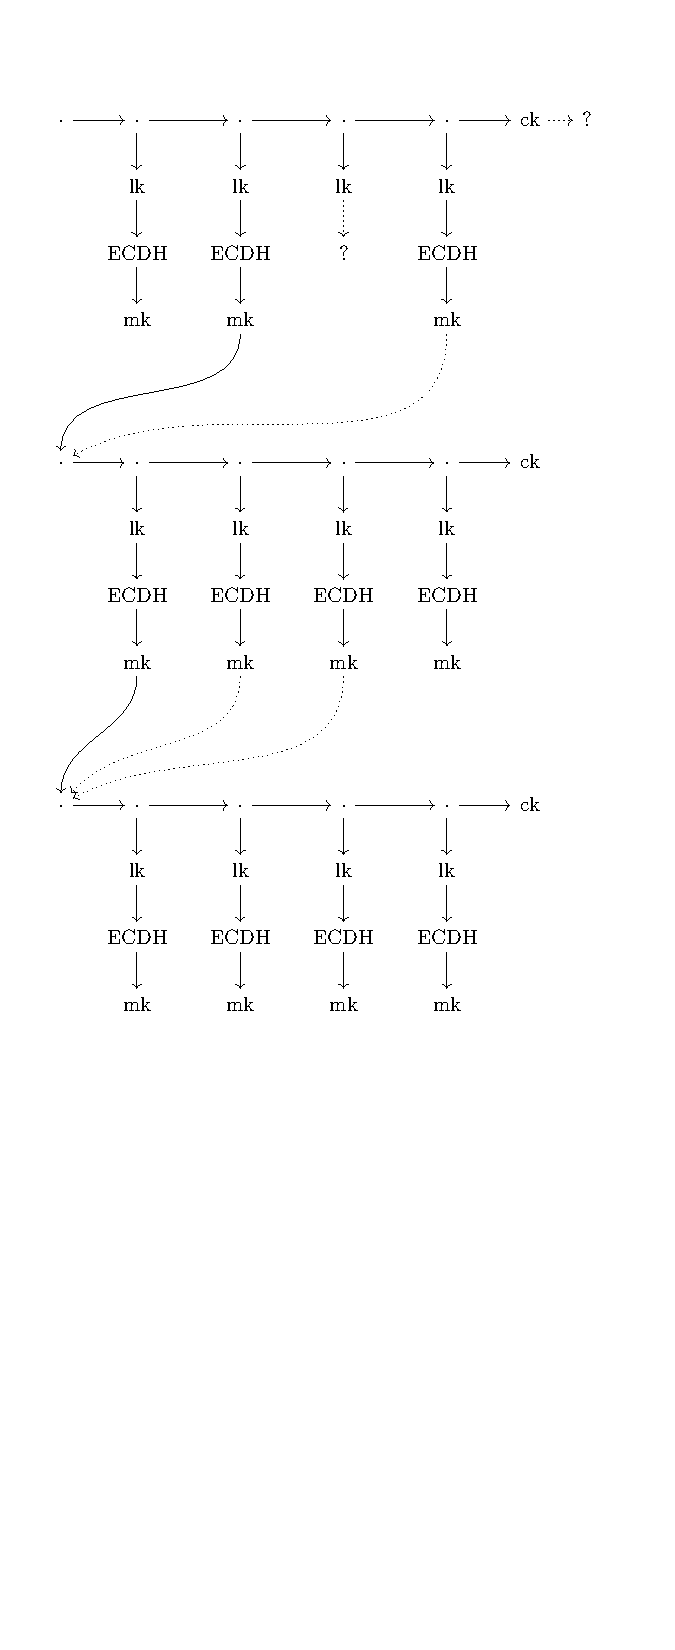
\includegraphics[width=\textwidth,trim={0 0 0 47},clip]{../up/32c3/Xolotl_diagram0}
\end{columns}
\end{frame}


\begin{frame}[t]{Tweaking Sphinx}
\begin{columns}[T]
\column{0.55\textwidth}

Not all hops need a ratchet, but \\
 \hspace*{1pt} ratchet hops must decrypt $\beta$ twice,
 \hspace*{1pt} requiring extra $\phi_j$. 

% \medskip

% We let $l$ differ for these virtual hops,
%  \hspace*{1pt} so terms like $i l$ become $\sum_{j=0}^i l_j$.

\medskip

Ratchet hops replace $s_i$ by $\textrm{mk}$ \\
 \hspace*{1pt} in blinding $\alpha$ or decrypting $\delta$, while \\
 \hspace*{1pt} non-ratchet hops remain the same.

\column{0.45\textwidth}
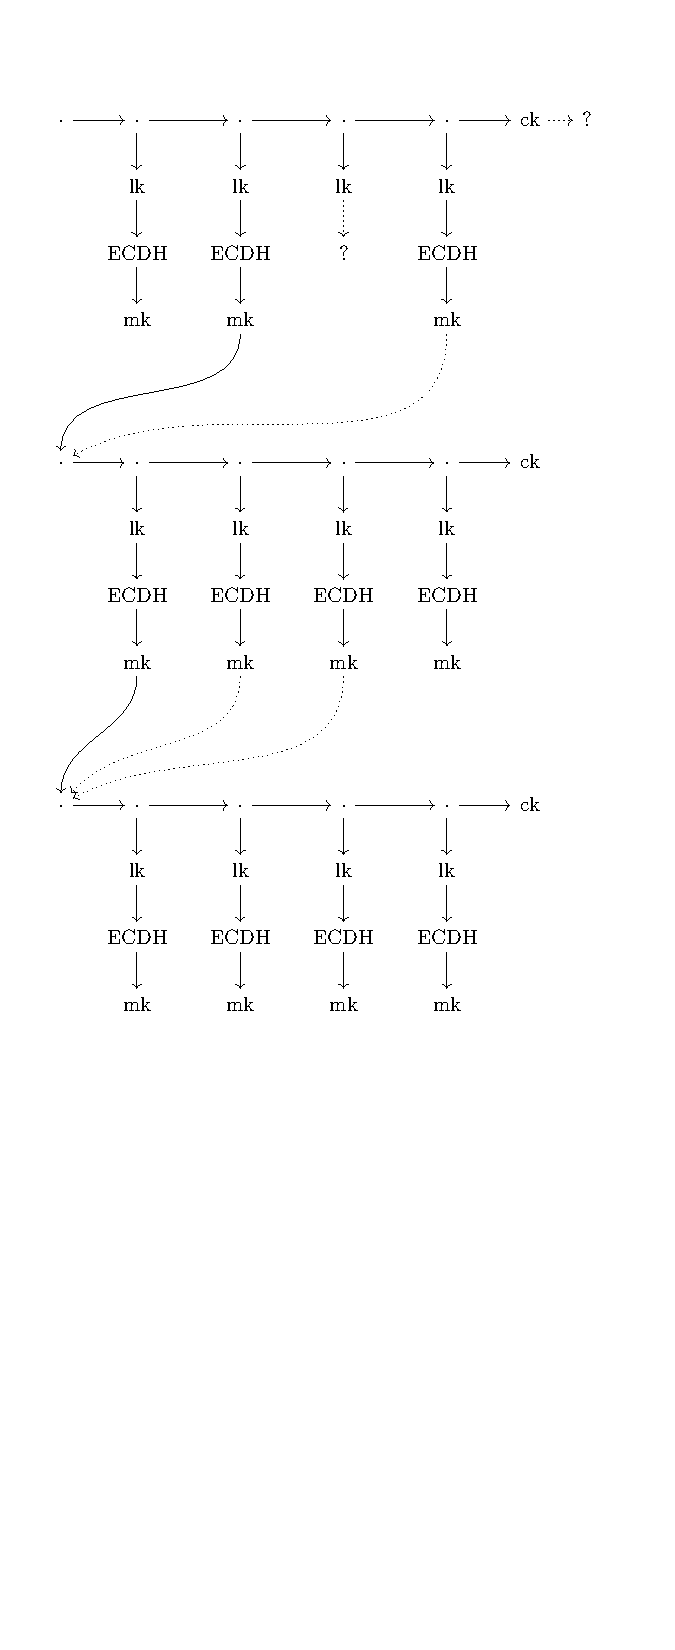
\includegraphics[width=\textwidth,trim={0 0 0 47},clip]{../up/32c3/Xolotl_diagram0}
\end{columns}
\end{frame}


\begin{frame}{Post-quantum?}
\begin{columns}[T]
\column{0.6\textwidth}
Ratchet hops improve key erasure, but..

\medskip

A quantum adversary can evolve all \\
 \hspace*{2pt} ratchets, including yours.

\medskip
\only<2>{
First, if ratchets live long enough, then \\
\hspace*{2pt} doing so might get expensive, \\
\hspace*{2pt} assuming ratchets names evolve.

\medskip

Second, we create new ratchets using \\
\hspace*{2pt} a post-quantum key exchange.

\smallskip

...}

\column{0.4\textwidth}
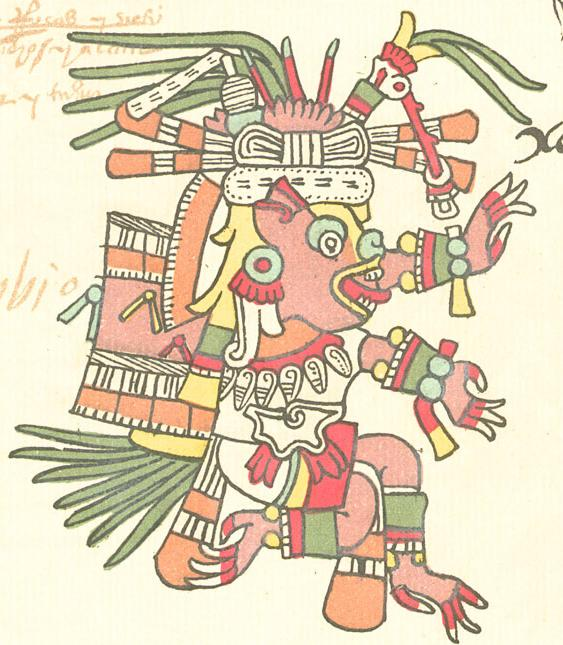
\includegraphics[width=1.2\textwidth]{../pics/Xolotl}
\end{columns}
\end{frame}


\begin{frame}{Aren't ratchet hops less anonymous?}

Isn't avoiding linking packets the whole point of Sphinx?

\medskip

A ratchet obviously links any two packets using it, \\
\hspace*{2pt} but that's no where near the end of the story.

\bigskip

First, we can judiciously intermix ratchet and non-ratchet hops.
\[ \textrm{User} \to \textrm{Guard} \to \textrm{Normal} \to \textrm{Ratchet} \to \textrm{Normal} \to \textrm{Cross} \to \cdots \]

\smallskip
Second, ratchets need not always be owned by the same user!

\end{frame}



\end{document}




% delivery : 32c3.tex


% \begin{frame}{?}
% \end{frame}




